\documentclass{scrartcl}
\usepackage{lipsum}
%%\usepackage[french]{babel}
%%\usepackage[ngerman]{babel}


%% Choose default font for the document
%% Warning : only ONE of the following should be enabled
\usepackage{kpfonts}
%%\usepackage{libertine}

%% The following chose the default language for the document and
%% use the default typography rules for the choosen language.
\usepackage{polyglossia}
\setdefaultlanguage{english}
%% \setdefaultlanguage{german}
%%\setdefaultlanguage{french}

\usepackage[backend=biber, style=ieee]{biblatex}
\addbibresource{template.bib}

\usepackage{graphicx}
\graphicspath{ {./ressources/images/} }

\usepackage{array}

\usepackage{listings}

\begin{document}
\title{Web Simulation of a Thymio Robot}
\date{\today}   %% or \date{01 november 2018}
\author{Quentin Flückiger (\texttt{flucq1@bfh.ch})}





\maketitle
\clearpage

Declaration of Authorship
\clearpage
\clearpage

Management Summary
\clearpage
\clearpage

\tableofcontents
\clearpage

\section{Introduction}

\section{Environment}

\subsection{Thymio}
\subsubsection{What is Thymio} 

Thymio is an educational robot that aims at improving early education (starting in primary school) in STEM (Science, Technology, Engineering and Mathematics), computational thinking, base computer science and researching the acknowledgment by kids of robots in their learning environment. The project also had technical aims, such as how to provide hardware modularity, fast reaction time amid perception and action, clear internal communication bus in a user-friendly way and streamline development for group robot, this includes direct changes to the robots’ programs and parallel debugging wirelessly, transparently and cheaply.
The Thymio project is based on a collaboration between the MOBOTS group from the Swiss Federal Institute of Technology in Lausanne (EPFL) and the Lausanne Arts School (ECAL). MOBOTS being the Miniature Mobile Robots Group, they are mainly focused around system design for small robots of the kind. It started with a strange-looking pile of components, that were assembled on any kind of support and holt the name of “Monsieur Patate” (Sir Potato), most likely due to its appearance, that saw life during the first workshop between the two contributors. After what the first “Thymio” was developed, it was a four-block robot that could be self-assembled, but not self-programmed as it was coming with pre-programmed behaviours. It was used as a user study to gather feedback from clients to know what features needed to be implemented on the Thymio II.


\begin{figure}[h!]
  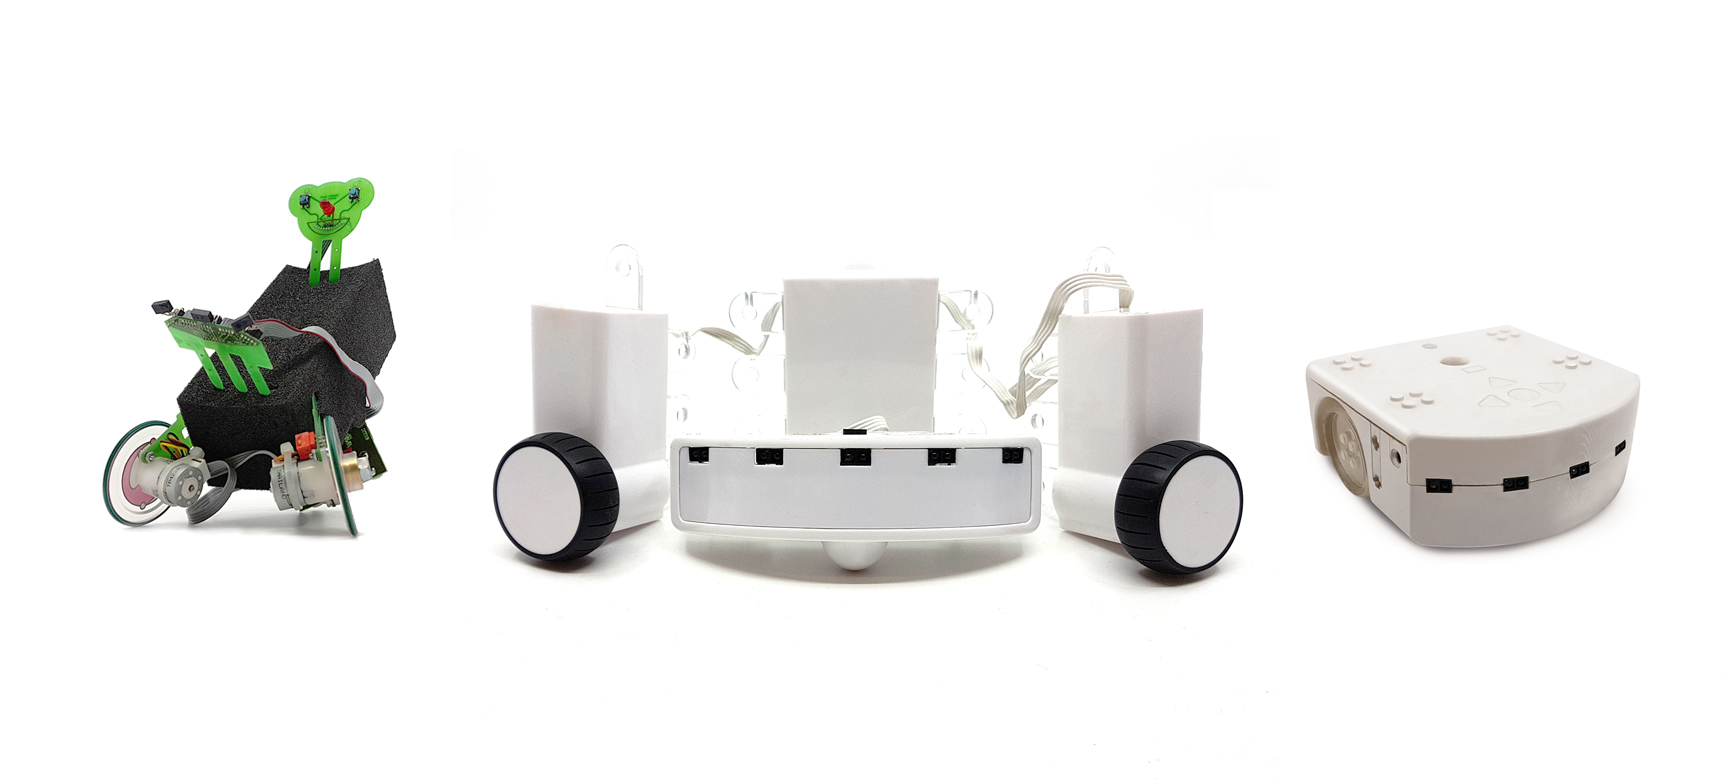
\includegraphics[width=\textwidth]{prototype_thymio_old}
  \caption{From left to right, "Monsieur Patate", Thymio, Thymio II}
  \label{fig:thymio_prototype}
\end{figure}

The result is a robot with a complex and complete set of sensors and actuators. The National Centre for Competence in Research (NCCR) Robotics research program supported the development of the robot whereas Mobsya, a non-profit organization that creates a robot, software, and educational activities to broaden young people’s mind about technology and science, oversees the production, distribution, and communication of said robot. Every step of the Thymio project is open-source and has a non-profit aim to enhance the quality of it with the user’s project and research, and reduce the cost and augment the lifetime for educational platforms and materials.

\begin{figure}[h!]
  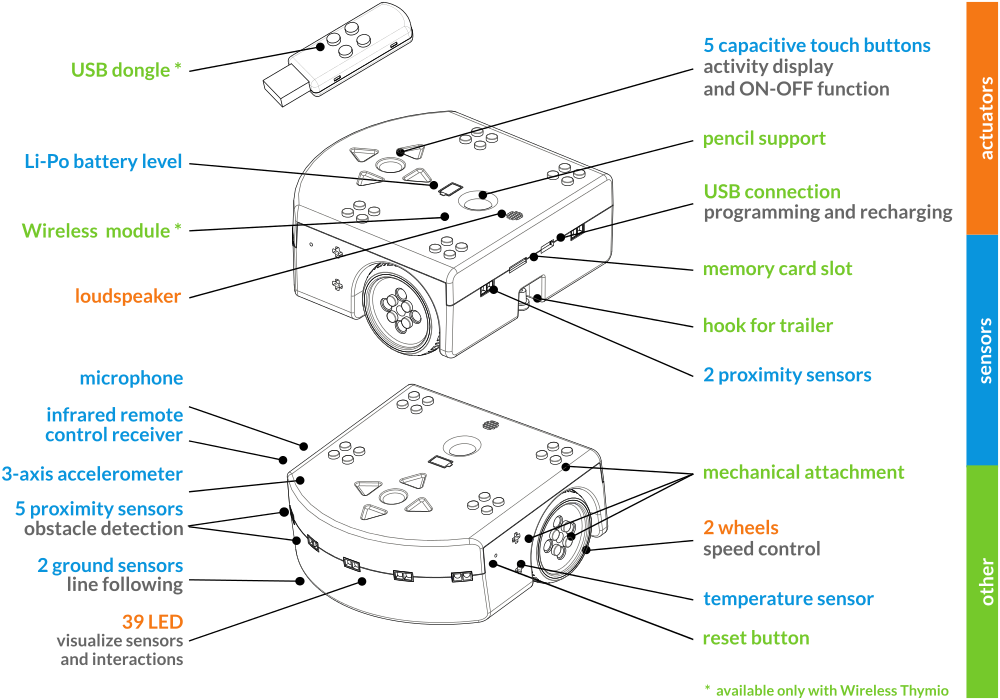
\includegraphics[width=\textwidth]{Wireless-thymioII-sensor-actuator-color-en}
  \caption{Thymio II sensor and actuator}
  \label{fig:thymio_sensor_actuator}
\end{figure}

\subsubsection{How does it works}

As seen in the figure above there exist two Thymio models, Thymio and Wireless Thymio. The difference between them lies in the ability of the second one to be programmed wirelessly, as its name suggests. To begin the creation of a program for the robot there exist two possibilities.
The first one, and the most common one for the public is done by using the software Aseba and a connected Thymio. In this case, the robot needs to be plugged in via USB cable or USB dongle (possible only if it is the Wireless Thymio) and powered on. Then the software can be used to connect to said robot and start to program in one of the four different programming languages, that are: VPL, Blockly, Aseba, and Scratch. Once the program is ready and sent to the robot it will be available to play.
The second option is to use the work-in-progress Thymio Suite version. This software doesn’t require a Thymio robot to be connected physically (or wirelessly) at all times as it has its own simulator built-in. The four said languages are still available, and one need to be chosen. After what comes the choice of connecting a physical Thymio or starting a simulation to emulate the programmed behaviour.

\subsubsection{The different programming languages}
\paragraph{VPL}
\paragraph{Blockly}
\paragraph{Aseba}
\paragraph{Scratch}
\subsubsection{What already exist} 
WeBots / Aseba logiciel
\subsection{TypeScript}
\subsection{Three JS}

For that we read the article book of \cite{Jerald:2015:VBH:2792790}
which is very interesting, much more than the article
\cite{Diniz:2017:UGO:3100317.3100324}

\section{Conclusion and future work}

\section{Appendices}
\subsection{Requirements Documentation}
\subsubsection{Vision}
\subsubsection{Objectives}
\subsubsection{System Boundaries}
\subsubsection{Requirements}

\subsection{Virtual Machine Configuration}
Step by step Guide on how to set it up and use it.

\subsection{Version control}

\subsection{Meetings}
\begin{tabular}{ | m{3cm} | m{10cm} | }
  \hline
  Date & Content \\
  \hline
  17.09.2019 & \textbf{Kick Off meeting}\\
  & Documentation/Management\\
  & Technology to use : ThreeJS and Typescript\\
  & Setting up the goals\\
  \hline
  24.09.2019 & \textbf{Second meeting} \\
  & Documentation language : English \\
  & Thymio model \\
  & Base talk about riks management \\
  \hline
  08.10.2019 & \textbf{Third meeting}\\
  & Workplace\\
  \hline
\end{tabular}

\listoffigures

\listoftables

\section{Problems encountered}
javascript not refreshing properly due to cache -> disable cache

%% Print the bibibliography and add the section to the table of content
\printbibliography[heading=bibintoc]

\end{document}
